\documentclass[border=3pt,tikz]{standalone}
\usepackage{amsmath}
\usetikzlibrary{calc}
\usetikzlibrary{arrows.meta} % for arrow size
\begin{document}
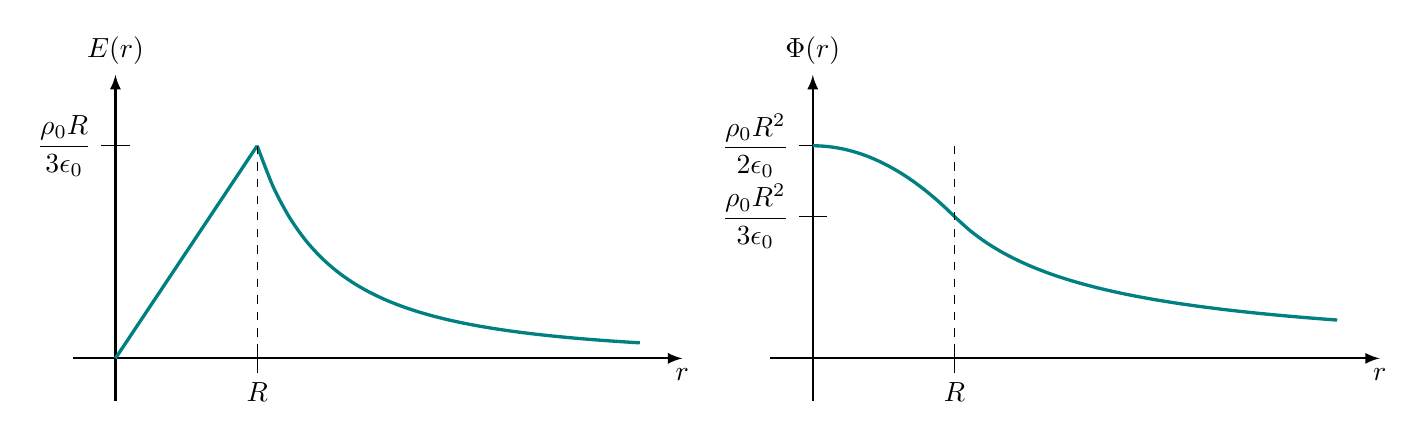
\begin{tikzpicture}[scale=1.8, rotate=0]
  \begin{scope}  
    \draw[thick, -latex] (-0.3, 0) -- (4, 0) node [below] {$r$};
    \draw[thick, -latex] (0, -0.3) -- (0, 2) node [above] {$E(r)$};
    \draw[very thick, teal] (0, 0) -- (1, 1.5);
    \draw[] (1, 0.1)-- (1, -0.1) node [below] {$R$};
    \draw[] (0.1, 1.5) -- (-0.1, 1.5) node [left] {$\dfrac{\rho_0 R}{3\epsilon_0}$};
    \draw[teal, very thick, domain=1:3.7, smooth, variable=\x,] plot ({\x}, {1.5/\x/\x});
    \draw[dashed] (1, 1.5) -- (1, 0);
  \end{scope}
  \begin{scope} [xshift=140]
    \draw[thick, -latex] (-0.3, 0) -- (4, 0) node [below] {$r$};
    \draw[thick, -latex] (0, -0.3) -- (0, 2) node [above] {$\Phi(r)$};
    \draw[] (1, 0.1)-- (1, -0.1) node [below] {$R$};
    \draw[] (0.1, 1.5) -- (-0.1, 1.5) node [left] {$\dfrac{\rho_0 R^2}{2\epsilon_0}$};
    \draw[] (0.1, 1) -- (-0.1, 1) node [left] {$\dfrac{\rho_0 R^2}{3\epsilon_0}$};
    \draw[teal, very thick, domain=0:1, smooth, variable=\x,] plot ({\x}, {1.5 -0.5*\x^2});
    \draw[teal, very thick, domain=1:3.7, smooth, variable=\x,] plot ({\x}, {1/\x});
    \draw[dashed] (1, 1.5) -- (1, 0);

  \end{scope}
  \end{tikzpicture}
\end{document}